%%%%%%%%%%%%%%%%%%%%%%%%%%%%%%%%%%%%%%%%%%%%%%%%%%%%%%%%%%%%%%%%%%%%%%%%%%%%%%%%
%%%%%%%%%%%%%%%%%%%%%%%%%%%%%%%%%%%%%%%%%%%%%%%%%%%%%%%%%%%%%%%%%%%%%%%%%%%%%%%%
%%                                                                            %%
%% kandidatarbetsbotten.tex versio 1.00 (2018/08/31)                          %%
%% by Henrik Wallen.                                                          %%
%% Opinnäytepohja käytettäväksi aaltothesis.sty (versio 3.20) -tyylitiedoston %%
%% kanssa.                                                                    %%
%% Toimiakseen paketti tarvitsee pdfx.sty v. 1.5.84 (2017/05/18) tai uudempi. %% 
%% The LaTeX template file to be used with the aaltothesis.sty (version 3.20) %%
%% style file.                                                                %%
%% This package requires pdfx.sty v. 1.5.84 (2017/05/18) or newer.            %% 
%%                                                                            %%
%% This is licensed under the terms of the MIT license below.                 %%
%%                                                                            %%
%% Copyright 2017-2018, by Luis R.J. Costa, luis.costa@aalto.fi,              %%
%% Copyright 2017-2018 Swedish translations in aaltothesis.cls by Elisabeth   %%
%% Nyberg, elisabeth.nyberg@aalto.fi and Henrik Wallén,                       %%
%% henrik.wallen@aalto.fi.                                                    %%
%% Copyright 2017-2018 Finnish documentation in the template opinnatepohja.tex%%
%% by Perttu Puska, perttu.puska@aalto.fi, and Luis R.J. Costa.               %%
%% Copyright 2018 English template thesistemplate.tex by Luis R.J. Costa.     %%
%% Copyright 2018 Swedish template kandidatarbetsbotten.tex by Henrik Wallen. %%
%%                                                                            %%
%% Permission is hereby granted, free of charge, to any person obtaining a    %%
%% copy of this software and associated documentation files (the "Software"), %%
%% to deal in the Software without restriction, including without limitation  %%
%% the rights to use, copy, modify, merge, publish, distribute, sublicense,   %%
%% and/or sell copies of the Software, and to permit persons to whom the      %%
%% Software is furnished to do so, subject to the following conditions:       %%
%% The above copyright notice and this permission notice shall be included in %%
%% all copies or substantial portions of the Software.                        %%
%% THE SOFTWARE IS PROVIDED "AS IS", WITHOUT WARRANTY OF ANY KIND, EXPRESS OR %%
%% IMPLIED, INCLUDING BUT NOT LIMITED TO THE WARRANTIES OF MERCHANTABILITY,   %%
%% FITNESS FOR A PARTICULAR PURPOSE AND NONINFRINGEMENT. IN NO EVENT SHALL    %%
%% THE AUTHORS OR COPYRIGHT HOLDERS BE LIABLE FOR ANY CLAIM, DAMAGES OR OTHER %%
%% LIABILITY, WHETHER IN AN ACTION OF CONTRACT, TORT OR OTHERWISE, ARISING    %%
%% FROM, OUT OF OR IN CONNECTION WITH THE SOFTWARE OR THE USE OR OTHER        %%
%% DEALINGS IN THE SOFTWARE.                                                  %%
%%                                                                            %%
%%                                                                            %%
%%%%%%%%%%%%%%%%%%%%%%%%%%%%%%%%%%%%%%%%%%%%%%%%%%%%%%%%%%%%%%%%%%%%%%%%%%%%%%%%
%%                                                                            %%
%% Botten för kandidatarbete på svenska. För mera instruktioner och modell på %%
%% finska och engelska se opinnäytepohja.tex och thesistemplate.tex.          %%
%%                                                                            %%
%%%%%%%%%%%%%%%%%%%%%%%%%%%%%%%%%%%%%%%%%%%%%%%%%%%%%%%%%%%%%%%%%%%%%%%%%%%%%%%%

%% OBS: Byt ut elec mot arts, biz, chem, eng eller sci om du inte är på ELEC
\documentclass[swedish, 12pt, a4paper, elec, utf8, a-2b, online]{aaltothesis}

\usepackage{graphicx}
\usepackage{amsmath,amsfonts,amssymb,amsbsy}

%% Korrigera ifall valet av högskola ovan inte automatiskt ger rätt texter
% \university{Aalto-univerisitetet}
% \school{Högskolan för elektroteknik}

%% Utbildningsprogram
\degreeprogram{Kandidatprogrammet i elektroteknik}

%% Huvudämne
\major{Elektronik och elektroteknik}

%% Huvudämnets kod
\code{ELEC3013}

\univdegree{BSc}

%% Namn
\thesisauthor{Teemu Teekkari}

%% Rubrik
\thesistitle{Botten för svenskspråkigt kandidatarbete}
%% Ifall rubriken inte ryms på en rad kan hända att radbytena inte blir
%% bra. Välj i så fall bättre radbyte(n) med hjälp av \\. I så fall måste
%% rubriken ges två gånger på följande sätt så att PDF/A-metadatan också
%% blir korrekt:
%\thesistitle[Kandidatarbetets rubrik ryms inte alltid på en rad]{Kandidatarbetets rubrik\\ryms inte alltid på en rad}


\place{Esbo}

%% Kandidatarbetets datum = presentationsdatum
%% För mellanversioner kan man istället använda respektive inlämningsdatum
\date{4.9.2018}

%% Huvudämnets ansvarslärare
\supervisor{Prof.\ Pirjo Professori}

%% Kandidatarbetets handledare. Typiskt en person, men det kan vara två.
\advisor{TkD Olli Ohjaaja}
%\advisor{DI Tina Tutkija}


%% Välj variant på Aalto-logon
%% \uselogo{aaltoRed|aaltoBlue|aaltoYellow|aaltoGray|aaltoGrayScale}{?|!|''}
\uselogo{aaltoRed}{!}


%% Nyckelord till sammanfattningsblanketten och PDF/A-metadatan
%% OBS: nyckelorden separeras med \spc -makron
\keywords{nyckelord\spc viktiga termer\spc centrala begrepp}

%% Sammanfattningens textdel utan styckeindelning (tomma rader) och
%% eventuella specialtecken. Denna version kommer i PDF/A-metadatan.
\thesisabstract{
  Sammanfattning av kandidatarbetet och dess viktigaste slutsatser. När
  sammanfattningen nedan är färdig: kopiera den hit och städa bort
  specialtecken och styckeindelning. 
}

%% Copyright-text
%% Syntax: \copyrigthtext{metadatatext}{text på sid 2}
\copyrighttext{Copyright \noexpand\copyright\ \number\year\ \ThesisAuthor}
{Copyright \copyright{} \number\year{} \ThesisAuthor}


%% Innehållet börjar
\begin{document}
	
%% Titelsidan
\makecoverpage

%% Copyright-sidan
%% Kan kommenteras bort, men det rekommenderas inte.
\makecopyrightpage

%% Sammanfattningen. Resten av informationen är definierad ovan. Här skrivs
%% själva texten. Låt bli att ha en tom rad (=nytt stycke) i början.

\begin{abstractpage}[swedish]
Sammandraget ska ge en koncis och heltäckande bild av arbetet. Skriv kort
om varje del, såsom syfte, metod, resultat och slutsatser. Dela in texten i
stycken men använd inga mellanrubriker. Använd inte heller tabeller,
figurer eller punktuppställningar och skriv inga källhänvisningar. Undvik
specialtecken. 

Notera också instruktionerna i källkoden (ovan) om hur man ser till att
sammandraget också kommer med i PDF/A-metadatan.

Om du skriver kandidatarbetet på svenska räcker det med ett svenskspåkigt
sammandrag enligt denna modell. I så fall är deft förmodligen lämpligt att
begränsa längden så att allt ryms på en sida.

Om du skriver ditt kandidatarbete på finska eller engelska, skriver du
mognadsprovet i form av ett svenskspråkigt sammandrag (abstrakt) av
kandidatarbetet. I så fall har du lämpligen två sammandrag i ditt färdiga
kandidatarbete: ett på arbetets språk och efter det ett på svenska, som då
är ditt mognadsprov. Längden ska i så fall vara minst 300--400 ord och det
kan hända att sammandraget (mognadsprovet) inte ryms på en sida.

\end{abstractpage}


%% Kandidatarbeten brukar inte ha förord. Se den finskspråkiga modellen
%% ifall du behöver ett.


%% Innehållsförteckning på en egen sida
\clearpage
\thesistableofcontents

%% Exempel på hur man gör en lista på symboler och förkortningar finns
%% också i den finskspråkiga modellen.

\clearpage
%% Här börjar själva sakinnehållet
%% 
\section{Inledning}

Detta dokument \texttt{kandidatarbetsbotten.tex} kan användas som
utgångspunkt för ett svenskspråkigt kandidatarbete. För layouten används
\texttt{aaltothesis.cls} som i sin tur använder
\texttt{aaltologo.sty}. Notera också att en relativt ny version av
\texttt{pdfx}-paketet behövs. Mera exempelkod och instruktioner finns i den
finskspråkiga mallen \texttt{opinnäytepohja.tex}. Se också vilka
instruktioner just ditt huvudämne har angående kandidatarbetets layout.


%% Det rekommenderas att varje nytt avsnitt (huvudrubrik) börjar på en ny
%% sida. Lägg alltså in en \clearpage före varje \section{...}
\clearpage
\section{Bakgrund}

Dela in ditt arbete i lämpliga stycken och avsnitt.

\subsection{Underrubrik}

Två nivåer med rubriker behövs ofta.

\subsubsection{Mindre rubrik}

Om det behövs finns det också en tredje rubriknivå.

\clearpage
\section{Exempelkod}

\subsection{Matematik}
\label{sec:matematik}

För exponentfunktionen $e^x$ eller $\exp(x)$ konvergerar potensserien
\begin{equation}
\label{eq:exp}
e^x = \sum_{n=0}^\infty\frac{x^n}{n!}
= 1 + x + ...
\end{equation}
för alla $x\in\mathbb C$. För $|x|\ll 1$ får man en bra approximation
med de två första termerna i~\eqref{eq:exp}.

Möjligheten att relativt snabbt och med bästa möjliga kvalitet
typsätta avancerade formler har alltid varit en av \LaTeX{}
styrkor. Läs kapitel 3 i~\cite{lshort} för att komma igång.

\subsection{Figurer}
\label{sec:figurer}

För att inkludera bilder använder man typiskt graphicx-paketet. Med
pdflatex kan man använda bilder i PDF-, PNG- och JPEG-format. \LaTeX{}
placerar figuren någonstans. Man kan ge önskemål med
placeringsargumenten t=top, b=bottom, p=page eller h=here, men det är
svårt att ha full kontroll på var figurer och tabeller placeras. Kom
ihåg att alltid hänvisa till figuren i texten!

\begin{figure}[t]
  \centering
  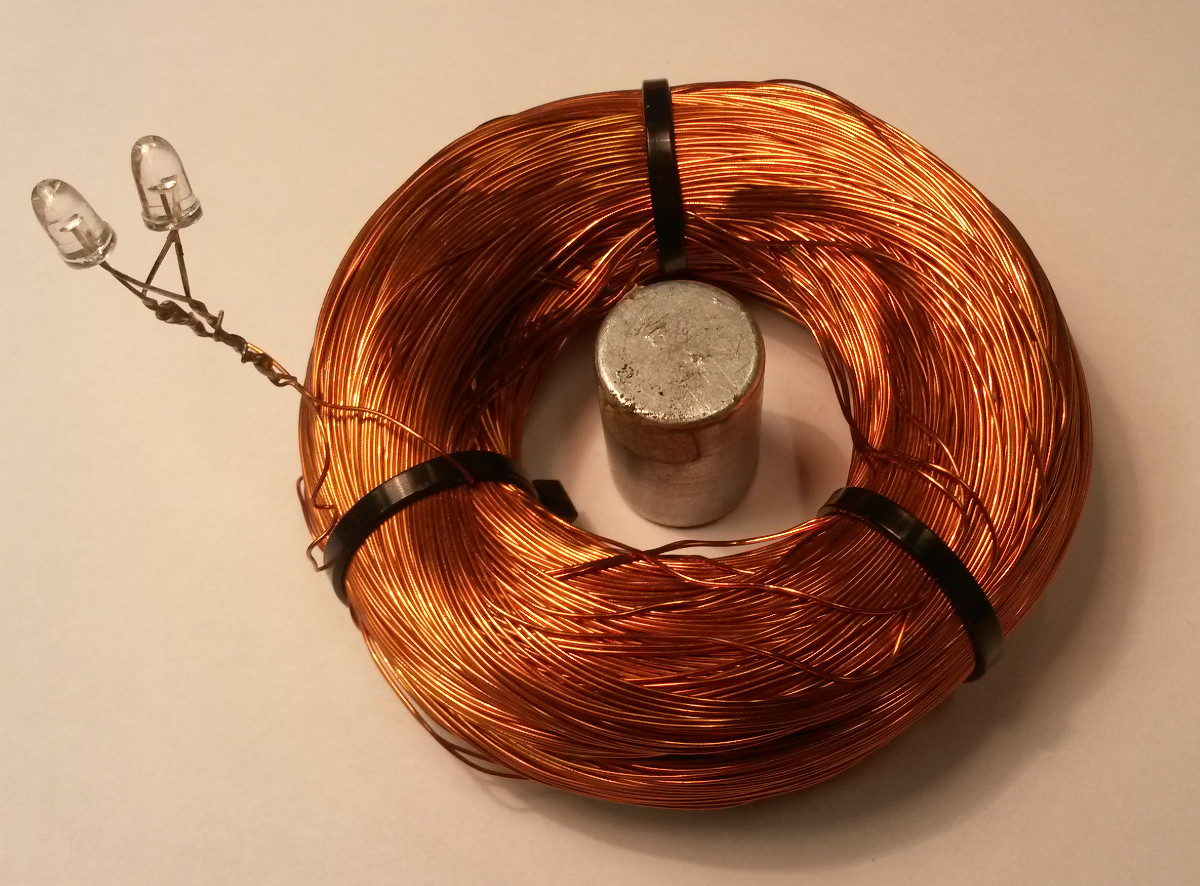
\includegraphics[width=0.5\textwidth]{ledspole.jpg}
  \caption{En spole för att demonstrera Faradays induktionslag.}
  \label{fig:spole}
\end{figure}

Med hjälp av utrustningen i figur~\ref{fig:spole} kan man demonstrera hur
ett föränderligt magnetfält inducerar en elektromotorisk kraft som i sin
tur ger upphov till en ström i spolen.

\subsection{Tabeller}
\label{sec:tabeller}

Tabeller fungerar lite på samma sätt som figurer, men notera att
tabelltexter placeras ovanför tabellen (i motsats till bildtexter som
placeras under bilden). Tabell~\ref{tab:bessel} innehåller några av
Besselfunktionens nollställen.

\begin{table}[t]
  \caption{Besselfunktionen nollställen $x_{ns}$
    för vilka $J_n(x_{ns})=0$.} 
  \label{tab:bessel}
  \begin{center}
    \begin{tabular}{c|ccc}
      n & $s=1$ & $s=2$ & $s=3$\\
      \hline
      0 & 2,405 & 5,520 & \phantom{0}8,654\\
      1 & 3,832 & 7,016 & 10,173\\
      2 & 5,136 & 8,417 & 11,620\\
      3 & 6,380 & 9,761 & 13,015
    \end{tabular}
  \end{center}
\end{table}

\subsection{Hänvisningar}

Man kan lite var som helst skapa en markör med \verb|\label{namn}| som
man hänvisar till med \verb|\ref{namn}|, vilket skriver ut siffran på
avsnitt, figur, tabell eller ekvation. Man kan också hänvisa till
sidnummer med \verb|\pageref{namn}|. För ekvationer använder man
hellre \verb|\eqref{namn}| så som i avsnitt~\ref{sec:matematik} där
potensserien~\eqref{eq:exp} hittas på sid~\pageref{eq:exp}. I koden
för avsnitt~\ref{sec:figurer} och~\ref{sec:tabeller} finns också
exempel på hänvisningar.

Notera förresten att man i allmänhet får köra (pdf)latex flere gånger för
att få alla hänvisningar rätt.

\subsection{Källhänvisningar}

För numrerade källhänvisningar och en kort referenslista är det enklaste
att skriva referenslistan för hand i \verb|thebibliography|-omgivningen,
och sen hänvisa med \verb|\cite| så som i detta exempel. För mera
omfattande referenslistor kan det löna sig att använda BibTeX för att få
rätt ordning och format på referenserna. I kombination med
\verb|natbib|-paketet kan man också använda källhänvisningar med författare
och årtal.

För en uttömmande, men ändå hyfsat kortfattad introduktion till och
referens för \LaTeX, se~\cite{lshort}. Kopka och Dalys
bok~\cite{kopka_daly} rekommenderas också varmt både som introduktion
och referensverk.

\clearpage
\section{Slutsatser}

Ett typiskt kandidatarbete är en litteraturstudie. Försök avsluta med några
egna slutsatser på basen av litteraturstudien. Det är ganska tråkigt att
bara sammanfatta arbetets innehåll.


%% Referensförteckningen

\clearpage
\thesisbibliography
\begin{thebibliography}{99}

\bibitem{lshort} T.\ Oetiker, H.\ Partl, I.\ Hyna, and E.\ Schlegl,
  \emph{The Not So Short Introduction to \LaTeX 2$\varepsilon$},
  Version 5.05, July 18, 2015,
  \url{http://mirrors.ctan.org/info/lshort/english/lshort.pdf}.

\bibitem{kopka_daly} H.\ Kopka and P.\ W.\ Daly, \emph{Guide to
    \LaTeX}, 4th Edition, Addison--Wesley Professional, 2003, ISBN:
  978-0321173850.

\end{thebibliography}

%% Se den finska modellen ifall du behöver appendix...

\end{document}
